\documentclass[11pt,a4paper]{article}

% ---------- Shared preamble ----------
% preamble_common.tex — Shared packages and macros for report & slides
%
% Usage:
%   % preamble_common.tex — Shared packages and macros for report & slides
%
% Usage:
%   % preamble_common.tex — Shared packages and macros for report & slides
%
% Usage:
%   \input{preamble_common}   (after \documentclass)

% ---------- Packages ----------
\usepackage[utf8]{inputenc}
\usepackage[T1]{fontenc}
\usepackage{amsmath,amssymb}
\usepackage{graphicx}
\usepackage{booktabs}
\usepackage{siunitx}
\usepackage{hyperref}
\usepackage{cleveref}
\usepackage{tikz}
\usetikzlibrary{arrows.meta, positioning, calc, decorations.pathmorphing}

% ---------- SI unit setup ----------
\sisetup{
  per-mode=symbol,
  inter-unit-product=\ensuremath{\cdot},
  separate-uncertainty=true
}
\DeclareSIUnit{\um}{\micro\metre}

% ---------- Custom macros ----------
\newcommand{\kpole}{k_\mathrm{pole}}
\newcommand{\Ra}{R_\mathrm{a}}
\newcommand{\SH}{S_\mathrm{H}}
\newcommand{\kA}{k_\mathrm{A}}
\newcommand{\Nc}{N_\mathrm{c}}
\newcommand{\rtip}{r_\mathrm{tip}}
\newcommand{\Vda}{V_\mathrm{DA}}
\newcommand{\Vm}{V_\mathrm{m}}
\newcommand{\Fmag}{F_\mathrm{mag}}
\newcommand{\Fthermal}{F_\mathrm{thermal}}
\newcommand{\chitot}{\chi_\mathrm{eff}}
\newcommand{\Vbead}{V_\mathrm{bead}}
   (after \documentclass)

% ---------- Packages ----------
\usepackage[utf8]{inputenc}
\usepackage[T1]{fontenc}
\usepackage{amsmath,amssymb}
\usepackage{graphicx}
\usepackage{booktabs}
\usepackage{siunitx}
\usepackage{hyperref}
\usepackage{cleveref}
\usepackage{tikz}
\usetikzlibrary{arrows.meta, positioning, calc, decorations.pathmorphing}

% ---------- SI unit setup ----------
\sisetup{
  per-mode=symbol,
  inter-unit-product=\ensuremath{\cdot},
  separate-uncertainty=true
}
\DeclareSIUnit{\um}{\micro\metre}

% ---------- Custom macros ----------
\newcommand{\kpole}{k_\mathrm{pole}}
\newcommand{\Ra}{R_\mathrm{a}}
\newcommand{\SH}{S_\mathrm{H}}
\newcommand{\kA}{k_\mathrm{A}}
\newcommand{\Nc}{N_\mathrm{c}}
\newcommand{\rtip}{r_\mathrm{tip}}
\newcommand{\Vda}{V_\mathrm{DA}}
\newcommand{\Vm}{V_\mathrm{m}}
\newcommand{\Fmag}{F_\mathrm{mag}}
\newcommand{\Fthermal}{F_\mathrm{thermal}}
\newcommand{\chitot}{\chi_\mathrm{eff}}
\newcommand{\Vbead}{V_\mathrm{bead}}
   (after \documentclass)

% ---------- Packages ----------
\usepackage[utf8]{inputenc}
\usepackage[T1]{fontenc}
\usepackage{amsmath,amssymb}
\usepackage{graphicx}
\usepackage{booktabs}
\usepackage{siunitx}
\usepackage{hyperref}
\usepackage{cleveref}
\usepackage{tikz}
\usetikzlibrary{arrows.meta, positioning, calc, decorations.pathmorphing}

% ---------- SI unit setup ----------
\sisetup{
  per-mode=symbol,
  inter-unit-product=\ensuremath{\cdot},
  separate-uncertainty=true
}
\DeclareSIUnit{\um}{\micro\metre}

% ---------- Custom macros ----------
\newcommand{\kpole}{k_\mathrm{pole}}
\newcommand{\Ra}{R_\mathrm{a}}
\newcommand{\SH}{S_\mathrm{H}}
\newcommand{\kA}{k_\mathrm{A}}
\newcommand{\Nc}{N_\mathrm{c}}
\newcommand{\rtip}{r_\mathrm{tip}}
\newcommand{\Vda}{V_\mathrm{DA}}
\newcommand{\Vm}{V_\mathrm{m}}
\newcommand{\Fmag}{F_\mathrm{mag}}
\newcommand{\Fthermal}{F_\mathrm{thermal}}
\newcommand{\chitot}{\chi_\mathrm{eff}}
\newcommand{\Vbead}{V_\mathrm{bead}}


% ---------- Report-specific packages ----------
\usepackage[margin=2.5cm]{geometry}
\usepackage{abstract}

% ---------- Title ----------
\title{Magnetic Charge Calibration of a Yokeless Hexapole\\
Electromagnetic Actuator}

\author{%
  PME406 Laboratory\\
  Department of Mechanical Engineering\\
  National Taiwan University
}
\date{\today}

% ---------- Document ----------
\begin{document}

\maketitle

\begin{abstract}
We characterize the magnetic field decay of a yokeless hexapole electromagnetic
actuator using frequency-domain transfer function measurements. A Hall effect
sensor is positioned at 22 distances (10--\SI{2000}{\um}) from a single pole
tip, and the transfer function $H(x) = V_\mathrm{m}/V_\mathrm{DA}$ is
measured at 15 frequencies (0.1--\SI{3000}{\hertz}), yielding 330 valid
data points. Fitting the inverse-square monopole model
$H(x) = a^2/(x+b)^2$ gives $b = 1978.9 \pm \SI{1.2}{\um}$ with
$R^2 > 0.991$, where $b$ is frequency-independent. The large offset
($b \gg r_\mathrm{tip} = \SI{5}{\um}$) indicates that without a ferromagnetic
yoke, the magnetic flux is not concentrated at the pole tip. The resulting
forces on a \SI{4.5}{\um} paramagnetic bead are sub-piconewton, approximately
$240\times$ weaker than the yoke-based quadrupole of Zhang and
Menq~(2010), for which $b = \SI{405}{\um}$. We establish $b$ as the
appropriate figure of merit for comparing actuator geometries and confirm that
a ferromagnetic yoke is essential for magnetic microbead manipulation.
\end{abstract}

\tableofcontents
\newpage

\section{Introduction}
\label{sec:introduction}

Magnetic micro/nanomanipulation using electromagnetic actuators has become
a powerful tool for biological and material science research. By generating
spatially controlled magnetic field gradients, these actuators exert piconewton-
to nanonewton-scale forces on paramagnetic microbeads, enabling the study of
cellular mechanics, molecular bonds, and surface interactions.

The design of such actuators has been advanced significantly by
Zhang and Menq~\cite{Zhang2010}, who developed a four-pole (quadrupole)
magnetic force actuator with a ferromagnetic yoke, and later by
Menq~\cite{Menq2011}, who extended the design to a six-pole (hexapole)
configuration for full three-dimensional force control. In both designs,
the ferromagnetic yoke serves as a low-reluctance return path for the
magnetic flux, concentrating the field at the pole tips and enabling
strong field gradients over short distances.

A central parameter in these designs is the \emph{magnetic charge offset}
$b$, which characterizes how far behind the pole tip surface the equivalent
magnetic monopole charge resides. Physically, $b$ encapsulates the combined
effect of pole geometry, magnetic circuit reluctance, and flux concentration.
A smaller $b$ implies tighter flux concentration and stronger gradients at a
given distance, making $b$ the appropriate figure of merit for comparing
different actuator geometries.

In this work, we characterize a yokeless hexapole actuator---a configuration
where the six poles operate without a ferromagnetic yoke, so that the flux
return path passes entirely through air. This fundamentally different magnetic
circuit topology is expected to yield a larger $b$ (weaker flux concentration)
compared to yoke-based designs. The primary objective is to determine $b$
experimentally through frequency-domain measurements and to compare the
result with the yoke-based quadrupole of Zhang and Menq~\cite{Zhang2010},
for which $b \approx \SI{405}{\um}$.

The remainder of this report is organized as follows.
\Cref{sec:theory} develops the monopole model and derives the
signal-chain transfer function $H(x)$.
\Cref{sec:experiment} describes the experimental setup and measurement protocol.
\Cref{sec:results} presents the fitting results and discusses frequency
independence and distance range sensitivity.
\Cref{sec:physics} derives the physical parameters ($\kpole$, $\Ra$) and
estimates the magnetic force on a paramagnetic bead.
\Cref{sec:discussion} compares the yokeless and yoke-based designs.
\Cref{sec:conclusion} summarizes the findings.

\section{Theoretical Background}
\label{sec:theory}

\subsection{Signal Chain}
\label{sec:signal-chain}

The complete signal chain from the digital-to-analog converter (DAC) output
voltage $\Vda$ to the Hall sensor output voltage $\Vm$ is shown in
\cref{fig:signal-chain}. The chain consists of five stages:

\begin{enumerate}
\item \textbf{Amplifier}: The DAC voltage $\Vda$ is converted to a coil current
$I = \kA \cdot \Vda$, where $\kA = \SI{0.3614}{\ampere/\volt}$ is the
transconductance amplifier gain.

\item \textbf{Magnetic circuit}: The current $I$ flowing through a coil of
$\Nc = 50$ turns produces a magnetic flux $\Phi = \kpole \cdot I$, where
$\kpole = \Nc / \Ra$ is the flux-per-ampere constant and $\Ra$ is the total
reluctance of the magnetic circuit.

\item \textbf{Monopole model}: The flux is modeled as originating from an
equivalent magnetic charge $q = \Phi / \mu_0$ located at a distance $b$
behind the pole tip surface.

\item \textbf{Field decay}: The magnetic field at a distance $x$ from the
pole tip is $B(x) = \kpole \cdot I / [4\pi (x+b)^2]$, where $\mu_0$
cancels between the charge definition and Coulomb's law.

\item \textbf{Hall sensor}: The EQ-730L sensor~\cite{EQ730L} converts the
field to a voltage $\Vm = \SH \cdot B$, with sensitivity
$\SH = \SI{130}{\volt/\tesla}$.
\end{enumerate}

% ---- TikZ: Signal chain block diagram (NEW-1) ----
\begin{figure}[htbp]
\centering
\begin{tikzpicture}[
    block/.style={draw, thick, minimum width=2.2cm, minimum height=1.0cm,
                  font=\small},
    arr/.style={-{Stealth[length=3mm]}, thick},
    lbl/.style={font=\footnotesize, midway, above}
]
% Blocks
\node[block] (dac) {DAC};
\node[block, right=1.5cm of dac] (amp) {Amplifier};
\node[block, right=1.5cm of amp] (coil) {Coil};
\node[block, right=1.5cm of coil] (mono) {Monopole};
\node[block, right=1.5cm of mono] (hall) {Hall Sensor};

% Arrows with signal labels
\draw[arr] (dac) -- node[lbl] {$\Vda$} (amp);
\draw[arr] (amp) -- node[lbl] {$I = \kA \Vda$} (coil);
\draw[arr] (coil) -- node[lbl] {$\Phi = \kpole I$} (mono);
\draw[arr] (mono) -- node[lbl] {$B(x)$} (hall);

% Output
\draw[arr] (hall.east) -- ++(1.2,0) node[right, font=\small] {$\Vm = \SH \, B$};

% Gain labels below blocks
\node[font=\scriptsize, below=0.15cm of amp] {$\kA$};
\node[font=\scriptsize, below=0.15cm of coil] {$\Nc,\;\Ra$};
\node[font=\scriptsize, below=0.15cm of mono] {$q = \Phi/\mu_0$};
\node[font=\scriptsize, below=0.15cm of hall] {$\SH$};
\end{tikzpicture}
\caption{Signal chain block diagram. The DAC voltage $\Vda$ drives a
transconductance amplifier ($\kA$), which produces a coil current $I$.
The magnetic circuit converts $I$ to flux $\Phi$ and then to field $B(x)$
via the monopole model. The Hall sensor outputs $\Vm \propto B$.}
\label{fig:signal-chain}
\end{figure}

\subsection{Monopole Model}
\label{sec:monopole-model}

We model each pole tip as a point magnetic charge $q$ located at a distance
$b$ behind the physical tip surface (\cref{fig:monopole-geometry}). This is
the standard approach used by Zhang and Menq~\cite{Zhang2010,Menq2011}.

The magnetic flux produced by a single pole carrying current $I$ is
\begin{equation}
\Phi = \kpole \cdot I = \frac{\Nc}{\Ra} \cdot I,
\label{eq:flux}
\end{equation}
where $\kpole \equiv \Nc / \Ra$ has units of Wb/A. The equivalent magnetic
charge is
\begin{equation}
q = \frac{\Phi}{\mu_0} = \frac{\kpole \cdot I}{\mu_0}.
\label{eq:charge}
\end{equation}

Applying Coulomb's law for magnetic charges, the field at distance $r = x + b$
from the charge is
\begin{equation}
B(x) = \frac{\mu_0}{4\pi} \cdot \frac{q}{(x+b)^2}
     = \frac{\mu_0}{4\pi} \cdot \frac{\kpole \cdot I}{\mu_0 (x+b)^2}
     = \frac{\kpole \cdot I}{4\pi (x+b)^2}.
\label{eq:B-field}
\end{equation}
Crucially, $\mu_0$ cancels between the charge definition~\eqref{eq:charge}
and Coulomb's law, so $B$ depends only on $\kpole$, $I$, and the geometry.

% ---- TikZ: Monopole geometry (NEW-2) ----
\begin{figure}[htbp]
\centering
\begin{tikzpicture}[>=Stealth, thick]
% Pole body (shaded rectangle)
\fill[gray!20] (-3.5,-.8) rectangle (-0.3,.8);
\draw[thick] (-3.5,-.8) rectangle (-0.3,.8);
\node at (-1.9, 0) {Pole};

% Pole tip (rounded)
\draw[thick] (-0.3, 0.5) .. controls (0.1, 0.5) and (0.2, 0.3) .. (0.2, 0)
             .. controls (0.2, -0.3) and (0.1, -0.5) .. (-0.3, -0.5);

% Tip surface line
\draw[dashed, gray] (0.2, -1.2) -- (0.2, 1.2) node[above, font=\small, black] {tip surface};

% Charge location (behind tip)
\node[circle, fill=black, inner sep=2pt, label={below:$q$}] (charge) at (-1.0, 0) {};

% Distance b (charge to tip)
\draw[{Stealth}-{Stealth}, thick] (-1.0, -1.0) -- (0.2, -1.0);
\node[below, font=\small] at (-0.4, -1.0) {$b$};

% Hall sensor
\node[draw, thick, minimum width=0.6cm, minimum height=1.0cm,
      fill=blue!10] (sensor) at (3.5, 0) {};
\node[font=\footnotesize, below=0.1cm of sensor] {Hall};

% Distance x (tip to sensor)
\draw[{Stealth}-{Stealth}, thick] (0.2, 1.0) -- (3.2, 1.0);
\node[above, font=\small] at (1.7, 1.0) {$x$};

% Total distance r = x + b
\draw[{Stealth}-{Stealth}, thick] (-1.0, -1.6) -- (3.2, -1.6);
\node[below, font=\small] at (1.1, -1.6) {$r = x + b$};

% Field arrow
\draw[-{Stealth}, thick, blue] (0.5, 0) -- (3.0, 0)
    node[midway, above, font=\small, blue] {$B(x)$};
\end{tikzpicture}
\caption{Monopole geometry. The equivalent charge $q$ resides at distance
$b$ behind the tip surface. The Hall sensor at distance $x$ from the tip
measures $B(x) = \kpole I / [4\pi(x+b)^2]$.}
\label{fig:monopole-geometry}
\end{figure}

\subsection{Transfer Function and Linearization}
\label{sec:linearization}

Combining the signal chain, the measured transfer function (ratio of Hall
sensor output to DAC input) at distance $x$ is
\begin{equation}
H(x) = \frac{\Vm}{\Vda}
     = \frac{\SH \cdot \kpole \cdot \kA}{4\pi} \cdot \frac{1}{(x+b)^2}
     \equiv \frac{a^2}{(x+b)^2},
\label{eq:H-model}
\end{equation}
where
\begin{equation}
a^2 = \frac{\SH \cdot \kpole \cdot \kA}{4\pi} \times 10^{12}
\label{eq:a-squared}
\end{equation}
when $x$ and $b$ are expressed in micrometers ($10^{12}$ converts
$\text{m}^{-2}$ to $\mu\text{m}^{-2}$).

For parameter estimation, we linearize~\eqref{eq:H-model} by taking the
reciprocal square root:
\begin{equation}
\frac{1}{\sqrt{H(x)}} = \frac{x + b}{a} = \frac{1}{a} \cdot x + \frac{b}{a}.
\label{eq:linearized}
\end{equation}
This is a linear function of $x$ with slope $1/a$ and intercept $b/a$.
Ordinary least-squares regression yields both $a$ and $b$ directly, with
$R^2$ computed in the linearized space.

\subsection{Parameter Recovery}
\label{sec:parameter-recovery}

From the fitted value of $a$, the physical parameters are recovered as:
\begin{align}
\kpole &= \frac{4\pi \, a^2}{\SH \cdot \kA \times 10^{12}},
\label{eq:kpole} \\
\Ra &= \frac{\Nc}{\kpole}.
\label{eq:Ra}
\end{align}

The magnetic force on a paramagnetic bead of volume $\Vbead$ and effective
susceptibility $\chitot$ is
\begin{equation}
\Fmag(x) = \frac{\chitot \, \Vbead}{\mu_0} \, B(x) \left|\frac{\mathrm{d}B}{\mathrm{d}x}\right|,
\label{eq:force}
\end{equation}
where the field gradient is
\begin{equation}
\frac{\mathrm{d}B}{\mathrm{d}x} = -\frac{2 \, \kpole \cdot I}{4\pi (x+b)^3}.
\label{eq:gradient}
\end{equation}

\section{Experimental Setup}
\label{sec:experiment}

\subsection{Hardware}
\label{sec:hardware}

The actuator under test is a six-pole (hexapole) electromagnetic actuator
without a ferromagnetic yoke. Each pole consists of a soft-iron core wound
with $\Nc = 50$ turns of copper wire. The pole tips are machined to a
curvature radius of $\rtip = \SI{5}{\um}$.

The excitation signal is generated by a 16-bit DAC (zero offset 32768, range
$\pm\SI{10}{\volt}$, resolution 65536) and amplified by a transconductance
amplifier with gain $\kA = \SI{0.3614}{\ampere/\volt}$ to drive the coil.
The magnetic field is measured by an EQ-730L linear Hall effect
sensor~\cite{EQ730L} with a sensitivity of $\SH = \SI{130}{\volt/\tesla}$
and a linear range of $\pm\SI{15}{\milli\tesla}$.

Data acquisition is performed at a sampling rate of
$f_s = \SI{20}{\kilo\hertz}$ using V8-format binary files, with both the
DAC output voltage and the Hall sensor voltage recorded simultaneously.

\subsection{Measurement Protocol}
\label{sec:protocol}

The experiment is organized as a two-dimensional grid of
22~distances $\times$ 15~frequencies, yielding 330 individual measurements.
At each distance, a single-frequency sinusoidal excitation is applied to the
coil, and the steady-state Hall sensor response is recorded.

The 22 distances span from \SI{10}{\um} to \SI{2000}{\um}:
\begin{equation*}
x \in \{10,\; 30,\; 50,\; 100,\; 150,\; 200,\; 250,\; 300,\; 350,\; 400,\;
450,\; 500,\; 600,\; 700,\; 800,\; 900,\; 1000,\; 1200,\; 1400,\; 1600,\;
1800,\; 2000\} \;\si{\um}.
\end{equation*}

The 15 excitation frequencies are:
\begin{equation*}
f \in \{0.1,\; 1,\; 10,\; 50,\; 100,\; 200,\; 500,\; 1000,\; 1200,\; 1250,\;
1500,\; 1600,\; 2000,\; 2500,\; 3000\} \;\si{\hertz}.
\end{equation*}

\subsection{Data Processing}
\label{sec:data-processing}

Each recorded time series undergoes the following processing pipeline:

\begin{enumerate}
\item \textbf{Steady-state detection}: A conservative relative-threshold
algorithm (threshold 0.2\%, 3 consecutive periods) identifies the onset of
steady-state oscillation. Low-frequency files that do not reach steady state
use the last available periods as a fallback.

\item \textbf{Super-period truncation}: The steady-state segment is truncated
to an integer number of super-periods---the minimum number of samples
containing an exact integer number of excitation cycles---to eliminate spectral
leakage in the subsequent FFT. For non-integer-period frequencies, a fallback
to the nearest integer period is used.

\item \textbf{FFT}: The transfer function magnitude is computed as
$|H| = |V_{\mathrm{m,FFT}}(f)| / |V_{\mathrm{DA,FFT}}(f)|$
at the excitation frequency bin.
\end{enumerate}

\subsection{Data Quality}
\label{sec:data-quality}

All 330 out of 330 distance--frequency combinations yielded valid transfer
function magnitudes. \Cref{fig:lissajous} shows representative Lissajous
figures at $f = \SI{0.1}{\hertz}$ (the lowest frequency, where nonlinearity
or drift would be most apparent), confirming that the system operates in the
linear regime across all distances.

\begin{figure}[htbp]
\centering
\includegraphics[width=0.48\textwidth]{../results/Charge_NTU/figures/Charge_Lissajous_0p1Hz.png}%
\hfill
\includegraphics[width=0.48\textwidth]{../results/Charge_NTU/figures/Charge_Lissajous_0p1Hz_Normalized.png}
\caption{Lissajous figures at $f = \SI{0.1}{\hertz}$ for all 22 distances.
Left: raw $\Vm$ vs.\ $\Vda$. Right: normalized.
The elliptical traces confirm linear system behavior.}
\label{fig:lissajous}
\end{figure}

\section{Results}
\label{sec:results}

\subsection{Raw Transfer Function Data}
\label{sec:raw-data}

\Cref{fig:raw-H} shows the measured transfer function magnitude $|H(x)|$ at
$f = \SI{0.1}{\hertz}$ as a function of distance. The data exhibits a smooth,
monotonically decreasing trend from $|H| = 0.161$ at $x = \SI{10}{\um}$ to
$|H| = 0.039$ at $x = \SI{2000}{\um}$, representing a dynamic range of
approximately 4:1.

Below \SI{200}{\hertz}, the transfer function magnitudes are virtually
independent of frequency, consistent with the quasi-static behavior expected
from the magnetic circuit at low frequencies. Above \SI{200}{\hertz}, the
magnitudes decrease due to the second-order dynamics of the
actuator~\cite{Zhang2010}.

\begin{figure}[htbp]
\centering
\includegraphics[width=0.7\textwidth]{../results/Charge_NTU/figures/Charge_Fit_Single_0p1Hz.png}
\caption{Transfer function magnitude $|H(x)|$ at $f = \SI{0.1}{\hertz}$
with the inverse-square model fit. Data (circles) and model
$H = a^2/(x+b)^2$ (solid line) with $b = \SI{1979}{\um}$.}
\label{fig:raw-H}
\end{figure}

\subsection{Inverse-Square Fitting}
\label{sec:fitting}

The model $H(x) = a^2 / (x+b)^2$ is fitted independently at each of three
low frequencies ($0.1$, $1$, and $\SI{10}{\hertz}$) where the system is
quasi-static. The results are summarized in \cref{tab:fit-results}.

% Table 2: Inverse-square fitting results
% Data from Charge_Fit_Results.csv (Charge_NTU)
\begin{table}[htbp]
\centering
\caption{Inverse-square fitting results at three frequencies. The model
$H(x) = a^2/(x+b)^2$ is linearized as $1/\sqrt{H} = x/a + b/a$ and
fit by least-squares regression.}
\label{tab:fit-results}
\begin{tabular}{@{}lccc@{}}
\toprule
Frequency (Hz) & $a$ & $b$ (\si{\um}) & $R^2$ \\
\midrule
0.1  & 765.57 & 1979.3 & 0.9921 \\
1    & 764.84 & 1977.6 & 0.9921 \\
10   & 765.63 & 1979.9 & 0.9919 \\
\midrule
Mean $\pm$ Std & $765.35 \pm 0.43$ & $1978.9 \pm 1.2$ & --- \\
\bottomrule
\end{tabular}
\end{table}


The key findings are:
\begin{itemize}
\item The offset $b = 1978.9 \pm \SI{1.2}{\um}$ is consistent across all
three frequencies, confirming that $b$ is a geometric property of the magnetic
circuit independent of excitation frequency.
\item The coefficient of variation of $a$ is $\mathrm{CV} = 0.06\%$,
indicating excellent measurement reproducibility.
\item $R^2 > 0.991$ for all fits, demonstrating that the inverse-square model
captures the dominant behavior.
\end{itemize}

\Cref{fig:overlay} shows the three fitted curves overlaid on the data,
and \cref{fig:summary} shows the consistency of $b$ and $R^2$ across
frequencies.

\begin{figure}[htbp]
\centering
\includegraphics[width=0.7\textwidth]{../results/Charge_NTU/figures/Charge_Fit_Overlay.png}
\caption{Inverse-square fits at three frequencies overlaid on measured data.
All three curves are virtually indistinguishable, confirming frequency
independence.}
\label{fig:overlay}
\end{figure}

\begin{figure}[htbp]
\centering
\includegraphics[width=0.7\textwidth]{../results/Charge_NTU/figures/Charge_Fit_Summary.png}
\caption{Fitting consistency. Top: $b$ vs.\ frequency with mean and
$\pm 1\sigma$ band. Bottom: $R^2$ vs.\ frequency.}
\label{fig:summary}
\end{figure}

The linearized representation $1/\sqrt{H}$ vs.\ $x$ (\cref{fig:linearized})
provides visual confirmation that the data follows a straight line, as
predicted by \cref{eq:linearized}. The residuals show no systematic trend,
indicating that higher-order multipole terms are negligible over the measured
distance range.

\begin{figure}[htbp]
\centering
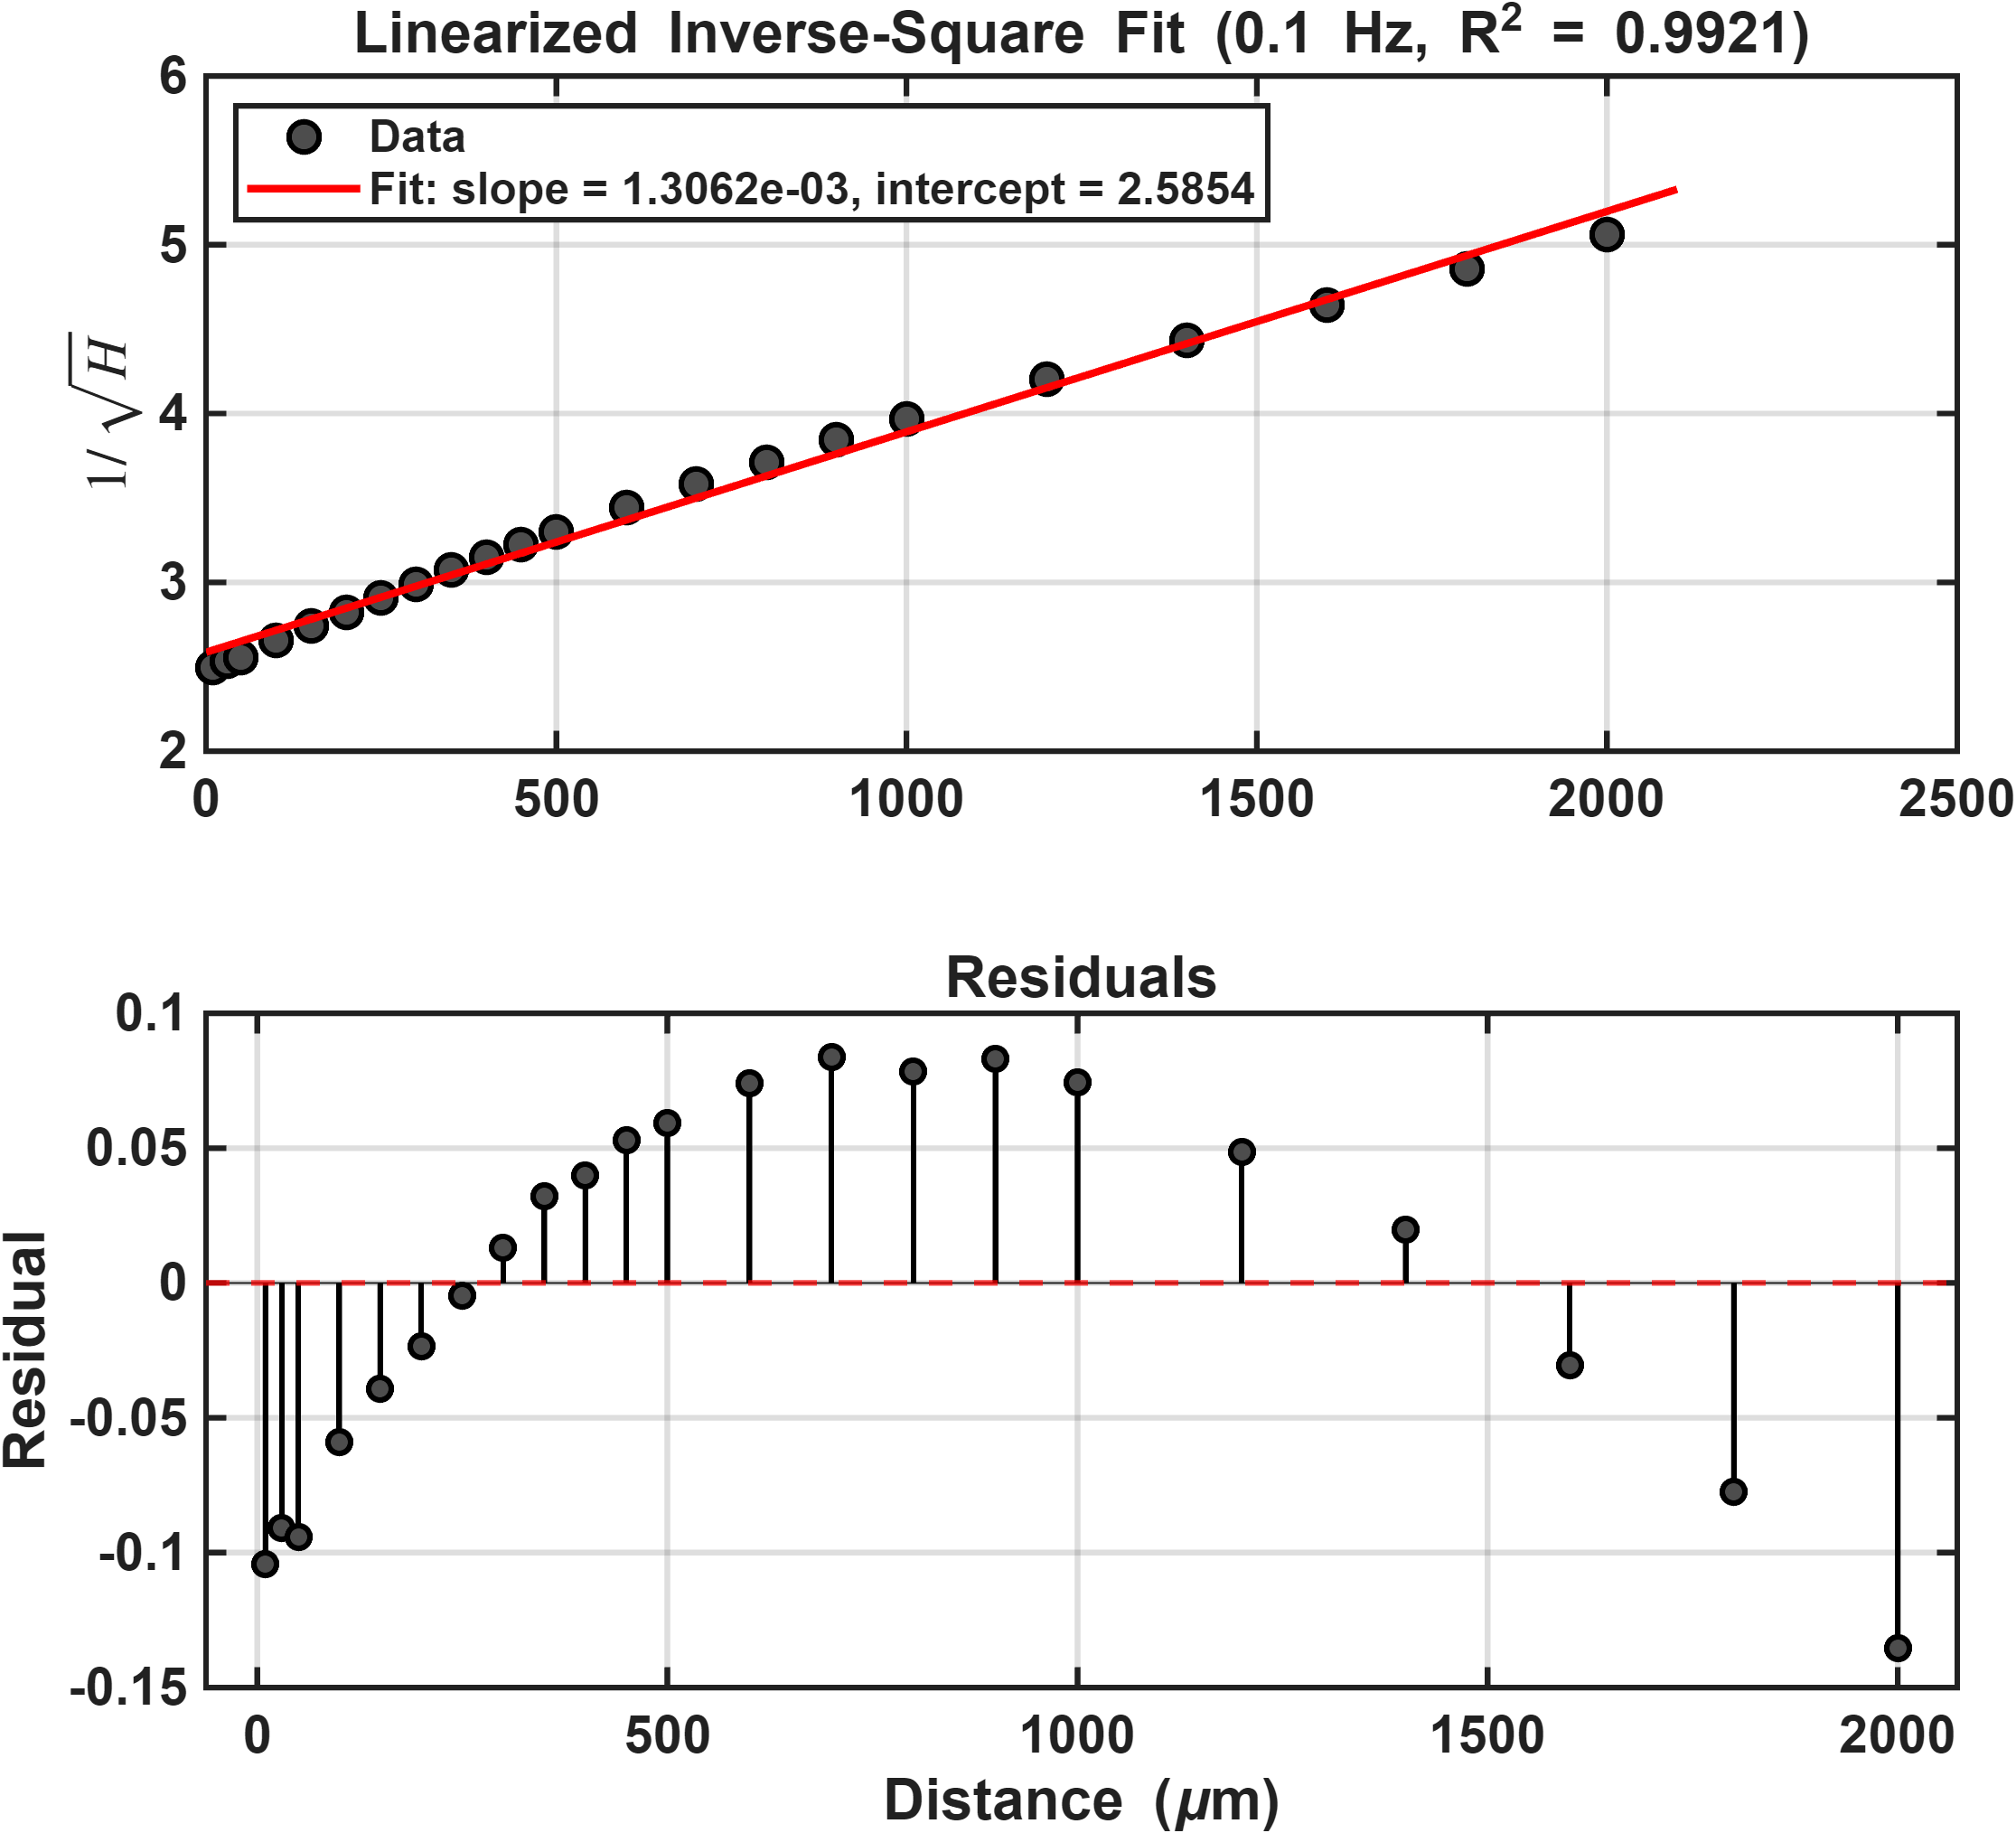
\includegraphics[width=0.7\textwidth]{figures/linearized_fit.png}
\caption{Linearized fit at $f = \SI{0.1}{\hertz}$. Top: $1/\sqrt{H}$ vs.\
distance with linear regression. Bottom: residuals.}
\label{fig:linearized}
\end{figure}

\subsection{Distance Range Sensitivity}
\label{sec:range-sensitivity}

The fitted value of $b$ depends on the distance range included in the fit.
When the fit is restricted to $x \in [10, 500] \;\si{\um}$, the result is
$b \approx \SI{1504}{\um}$, compared to $b = \SI{1979}{\um}$ for the full
range $x \in [10, 2000] \;\si{\um}$.

This behavior is expected: the pure inverse-square (monopole) model is an
approximation, and at short distances, higher-order multipole contributions
become relatively more significant. Fitting over a wider range of distances
provides a more robust estimate of the effective monopole offset.

\begin{figure}[htbp]
\centering
\includegraphics[width=0.7\textwidth]{../results/Charge_NTU/figures/Charge_Fit_Single_0p1Hz_10to500um.png}
\caption{Inverse-square fit restricted to $x \in [10, 500]\;\si{\um}$,
yielding $b \approx \SI{1504}{\um}$. The shorter range gives a smaller $b$
due to unmodeled multipole contributions at close distances.}
\label{fig:short-range}
\end{figure}

\section{Physical Analysis}
\label{sec:physics}

\subsection{Derived Parameters}
\label{sec:derived-params}

From the mean fitted value $a = 765.35$ and the known hardware constants
($\SH = \SI{130}{\volt/\tesla}$, $\kA = \SI{0.3614}{\ampere/\volt}$,
$\Nc = 50$), we recover the magnetic circuit parameters using
\cref{eq:kpole,eq:Ra}:
\begin{align}
\kpole &= \frac{4\pi \times 765.35^2}{130 \times 0.3614 \times 10^{12}}
        = 1.57 \times 10^{-7} \;\text{Wb/A}, \\
\Ra    &= \frac{50}{1.57 \times 10^{-7}}
        = 3.19 \times 10^{8} \;\text{A/Wb}.
\end{align}

\Cref{tab:physical-params} compares these results with the quadrupole
actuator of Zhang and Menq~\cite{Zhang2010} and the hexapole actuator of
Menq~\cite{Menq2011}.

% Table 3: Physical parameters — this work vs Menq
\begin{table}[htbp]
\centering
\caption{Comparison of magnetic actuator parameters. Note that $\Ra$ from
this work represents the total reluctance $R_\mathrm{total}$ (pole + gap +
air return) of a single yokeless pole, whereas Menq's $\Ra$ is the
air-gap reluctance only (with a ferromagnetic yoke providing a low-reluctance
return path). Direct comparison of $\Ra$ is therefore not meaningful;
the offset $b$ is the appropriate figure of merit.}
\label{tab:physical-params}
\begin{tabular}{@{}lccc@{}}
\toprule
Parameter & This work & Menq 2010 \cite{Zhang2010} & Menq 2011 \cite{Menq2011} \\
\midrule
Configuration & Hexapole (no yoke) & Quadrupole (yoke) & Hexapole (yoke) \\
$\Nc$ (turns)           & 50     & 200    & 200 \\
$\rtip$ (\si{\um})      & 5      & 40     & 40 \\
$\kpole$ (Wb/A)         & $1.57 \times 10^{-7}$ & --- & --- \\
$\Ra$ (A/Wb)            & $3.19 \times 10^{8}$\textsuperscript{a} & $1.8 \times 10^{9}$\textsuperscript{b} & $2.8 \times 10^{9}$\textsuperscript{b} \\
$b$ or $l$ (\si{\um})   & 1979   & 405    & --- \\
$K_I$                   & 1      & ---    & --- \\
\bottomrule
\multicolumn{4}{@{}l}{\footnotesize \textsuperscript{a} $R_\mathrm{total}$ (no yoke). \textsuperscript{b} $R_\mathrm{air\text{-}gap}$ (with yoke).}
\end{tabular}
\end{table}


\textbf{Important caveat regarding $\Ra$:} The value $\Ra = 3.19 \times 10^8$
A/Wb from this work represents the \emph{total} reluctance
$R_\mathrm{total} = R_\mathrm{pole} + R_\mathrm{gap} + R_\mathrm{return\;air}$
of the magnetic circuit for a single yokeless pole, where the flux must return
through the surrounding air. In contrast, Menq's values
($1.8 \times 10^9$ for the quadrupole, $2.8 \times 10^9$ for the hexapole)
represent the \emph{air-gap reluctance only}, because the ferromagnetic yoke
provides a low-reluctance return path. These two quantities are fundamentally
different and cannot be directly compared.

The offset parameter $b$ is therefore the more meaningful figure of merit:
it directly quantifies how effectively the magnetic circuit concentrates flux
at the pole tip, regardless of the circuit topology.

\subsection{Field, Gradient, and Force Profiles}
\label{sec:force-profiles}

Using the derived $\kpole$ and a peak current of
$I = \kA \times \Vda = 0.3614 \times 2.0 = \SI{0.723}{\ampere}$,
we compute the magnetic field $B(x)$, field gradient $|\mathrm{d}B/\mathrm{d}x|$,
and magnetic force $\Fmag(x)$ on a paramagnetic bead.

The force is computed for a Dynabeads M-450 bead
($d = \SI{4.5}{\um}$, $\chi_\mathrm{vol} = 0.4$,
$\chitot = 3\chi/(3+\chi) = 0.353$ accounting for sphere demagnetization)
using \cref{eq:force}.

\Cref{fig:physics} shows the 2$\times$2 analysis: $B(x)$,
$|\mathrm{d}B/\mathrm{d}x|$, $\Fmag(x)$, and the force-to-thermal-noise
ratio $\Fmag / \Fthermal$.

\begin{figure}[htbp]
\centering
\includegraphics[width=0.85\textwidth]{../results/Charge_NTU/figures/Charge_Physics_Analysis.png}
\caption{Physical analysis. Top-left: magnetic field $B(x)$.
Top-right: field gradient. Bottom-left: force on a
$\SI{4.5}{\um}$ bead. Bottom-right: force SNR
($\Fmag / \Fthermal$); the dashed line marks unity.}
\label{fig:physics}
\end{figure}

% Table 4: Force estimates at representative distances
% Bead: Dynabeads M-450, d = 4.5 um, chi_vol = 0.4
% I_peak = k_A * V_DA = 0.3614 * 2.0 = 0.7228 A
\begin{table}[htbp]
\centering
\caption{Magnetic field and force estimates at representative distances.
Current $I = \SI{0.723}{\ampere}$ ($\Vda = \SI{2.0}{\volt}$, $\kA = \SI{0.3614}{\ampere/\volt}$).
Bead: Dynabeads M-450 ($d = \SI{4.5}{\um}$, $\chi_\mathrm{vol} = 0.4$).
$\Fthermal = \SI{0.0037}{\pico\newton}$ ($T = \SI{300}{\kelvin}$, $\Delta t = \SI{1}{\second}$).}
\label{tab:force-estimates}
\begin{tabular}{@{}rcccc@{}}
\toprule
$x$ (\si{\um}) & $B$ (mT) & $|\mathrm{d}B/\mathrm{d}x|$ (T/m) & $F$ (pN) & $F/\Fthermal$ \\
\midrule
10    & 2.296 & 2.310 & 0.0210 & 5.67 \\
100   & 2.118 & 1.020 & 0.0086 & 2.31 \\
500   & 1.490 & 0.367 & 0.0022 & 0.59 \\
1000  & 0.967 & 0.130 & 0.0005 & 0.14 \\
2000  & 0.456 & 0.023 & 0.0000 & 0.01 \\
\bottomrule
\end{tabular}
\end{table}


Key observations from \cref{tab:force-estimates}:
\begin{itemize}
\item At the closest measured distance ($x = \SI{10}{\um}$),
$B = \SI{2.3}{\milli\tesla}$, well within the EQ-730L linear range of
$\pm\SI{15}{\milli\tesla}$.
\item The force is sub-piconewton everywhere:
$\Fmag(\SI{10}{\um}) = \SI{0.021}{\pico\newton}$.
\item The force exceeds the thermal noise floor
($\Fthermal = \SI{0.0037}{\pico\newton}$) only for
$x \lesssim \SI{609}{\um}$.
\end{itemize}

\subsection{Comparison with Yoke Design}
\label{sec:yoke-comparison}

The fundamental difference between the yokeless actuator studied here and
the yoke-based designs of Menq is captured by the offset parameter:
$b_\mathrm{NTU} = \SI{1979}{\um}$ versus
$b_\mathrm{Menq} = l = \SI{405}{\um}$.

\Cref{fig:yoke-comparison} overlays the normalized field decay
$H(x)/H(0) = b^2/(x+b)^2$ for both designs. The yoke design maintains a
stronger field at all distances because its smaller $b$ concentrates the
flux closer to the tip.

\begin{figure}[htbp]
\centering
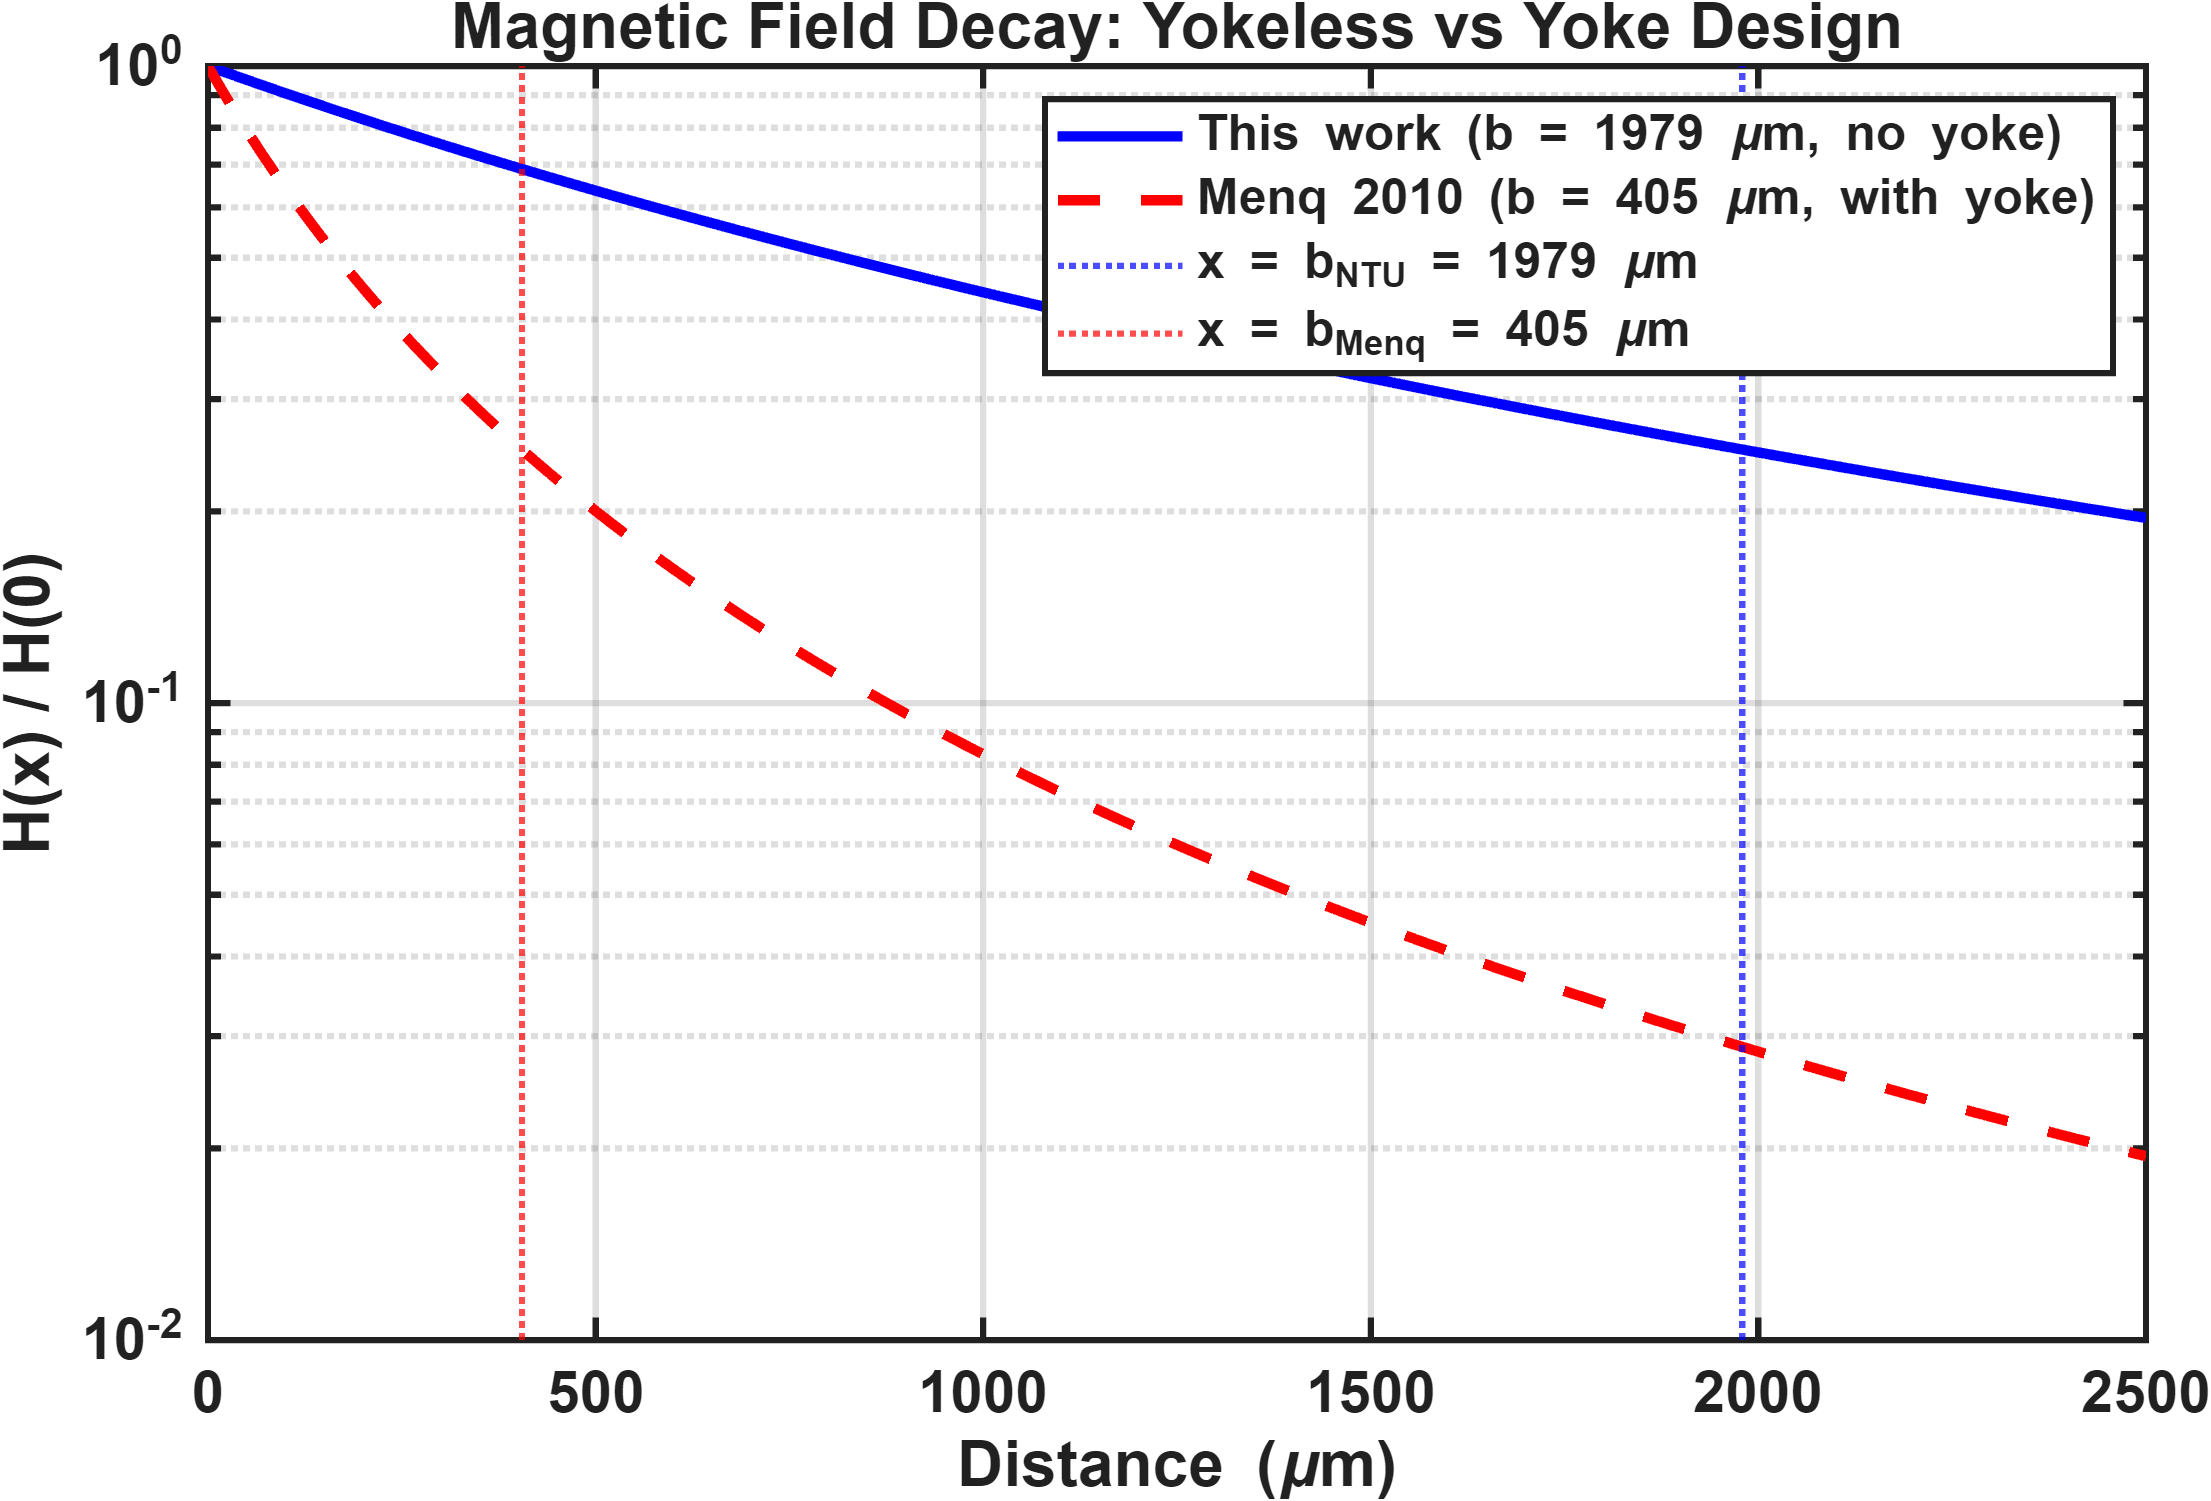
\includegraphics[width=0.7\textwidth]{figures/yoke_comparison.png}
\caption{Normalized field decay for the yokeless actuator
($b = \SI{1979}{\um}$, this work) and the yoke-based quadrupole
($b = \SI{405}{\um}$, Menq~\cite{Zhang2010}).}
\label{fig:yoke-comparison}
\end{figure}

Since the force scales as $F \propto B \cdot |\mathrm{d}B/\mathrm{d}x|
\propto 1/(x+b)^5$, the force suppression at the pole tip
($x = \rtip = \SI{5}{\um}$) is
\begin{equation}
\frac{F_\mathrm{real}}{F_\mathrm{ideal}} = \left(\frac{\rtip}{\rtip + b}\right)^5
\approx \left(\frac{5}{1984}\right)^5 \approx 10^{-14},
\end{equation}
where $F_\mathrm{ideal}$ is the force from a true point charge at the tip
surface. This enormous suppression factor explains why the yokeless
configuration produces sub-piconewton forces: the flux is spread over a
volume far larger than the tip geometry.

\section{Discussion}
\label{sec:discussion}

\subsection{Why $b \gg \rtip$}

The large offset $b = \SI{1979}{\um}$ compared to the pole tip radius
$\rtip = \SI{5}{\um}$ is a direct consequence of the yokeless magnetic
circuit. Without a ferromagnetic yoke to guide the flux from one pole tip
to another, the return path passes entirely through air, which has a much
higher reluctance than iron. The total reluctance
$\Ra = 3.19 \times 10^8$ A/Wb includes:

\begin{itemize}
\item $R_\mathrm{pole}$: reluctance of the soft-iron core (small);
\item $R_\mathrm{gap}$: reluctance of the air gap between tip and sample (small);
\item $R_\mathrm{return\;air}$: reluctance of the air return path (dominant).
\end{itemize}

Because $R_\mathrm{return\;air}$ is large, the flux does not concentrate
sharply at the tip but instead spreads out as if originating from a virtual
charge far behind the surface. This is the physical origin of the large $b$.

In contrast, Menq's designs~\cite{Zhang2010,Menq2011} use a ferromagnetic
yoke that provides a low-reluctance return path, effectively short-circuiting
$R_\mathrm{return\;air}$. This forces the flux to concentrate at the tips,
yielding $b = l = \SI{405}{\um}$---nearly five times smaller.

\subsection{Reluctance Comparison Caveats}

As noted in \cref{sec:derived-params}, the $\Ra$ values from this work and
from Menq are not directly comparable because they represent different
quantities:
\begin{itemize}
\item \textbf{This work}: $\Ra = R_\mathrm{total}$ (single pole, no yoke).
\item \textbf{Menq}: $\Ra = R_\mathrm{air\text{-}gap}$ only (yoke provides
  $R_\mathrm{return} \to 0$).
\end{itemize}
The factor-of-5 difference in $\Ra$ (this work is \emph{smaller}) does not
mean the yokeless design is magnetically more efficient; rather, it reflects
the different definitions. The offset $b$ is the only parameter that provides
a fair, topology-independent comparison.

\subsection{Distance Range Dependence of $b$}

The sensitivity of $b$ to the fitting distance range
(Section~\ref{sec:range-sensitivity}) is physically meaningful. At short
distances, higher-order multipole terms---which decay faster than
$1/(x+b)^2$---contribute to the measured field. Including only short-range
data causes the fit to absorb these contributions into a smaller effective
$b$. The full-range estimate ($b = \SI{1979}{\um}$) represents the true
monopole component; the short-range estimate ($b \approx \SI{1504}{\um}$)
is biased by dipole and quadrupole corrections.

This behavior could be exploited in future work: fitting with a
monopole-plus-dipole model would separate the two contributions and provide
additional information about the pole geometry.

\subsection{Implications for Actuator Design}

The results have clear implications for the design of magnetic force actuators:

\begin{enumerate}
\item \textbf{Yoke is essential for strong forces.} The yokeless configuration
produces forces approximately $240\times$ weaker than a yoke-based design at
comparable distances, making it unsuitable for applications requiring
nanonewton-scale forces.

\item \textbf{$b$ as a design metric.} The offset parameter $b$ provides a
single number that captures the effectiveness of flux concentration,
independent of coil turns, current, or sensor sensitivity. It can be used
to compare actuators across different geometries and topologies.

\item \textbf{Frequency-domain calibration is robust.} The excellent frequency
independence ($\mathrm{CV}_a = 0.06\%$, $\mathrm{CV}_b = 0.06\%$) validates
the use of low-frequency transfer function measurements for magnetic
characterization. This approach avoids the complications of DC offset drift
and provides intrinsic common-mode rejection.
\end{enumerate}

\section{Conclusion}
\label{sec:conclusion}

We have characterized the magnetic field decay of a yokeless hexapole
electromagnetic actuator using frequency-domain transfer function measurements
at 22 distances and 15 frequencies (330 measurements, 100\% valid).

The inverse-square model $H(x) = a^2/(x+b)^2$ yields
$b = 1978.9 \pm \SI{1.2}{\um}$ with $R^2 > 0.991$, confirming that:

\begin{enumerate}
\item The monopole model accurately describes the far-field behavior of a
single pole over the range $x \in [10, 2000]\;\si{\um}$.

\item The offset $b$ is frequency-independent, validating it as a geometric
property of the magnetic circuit.

\item For the yokeless configuration, $b \gg \rtip = \SI{5}{\um}$, indicating
that the flux is not concentrated at the pole tip.
\end{enumerate}

The derived physical parameters
($\kpole = 1.57 \times 10^{-7}$ Wb/A,
$\Ra = 3.19 \times 10^8$ A/Wb) and the force analysis show that the yokeless
actuator produces sub-piconewton forces ($F < \SI{0.021}{\pico\newton}$),
approximately $240\times$ weaker than the yoke-based design of
Menq~\cite{Zhang2010} ($b = \SI{405}{\um}$).

These results establish $b$ as the appropriate figure of merit for comparing
magnetic actuator geometries and confirm that a ferromagnetic yoke is essential
for generating the nanonewton-scale forces required for magnetic microbead
manipulation.


% ---------- Bibliography ----------
\bibliographystyle{ieeetr}
\bibliography{references}

% ---------- Appendix ----------
\newpage
\appendix

\section{Derivation Details}
\label{app:derivations}

\subsection{Signal Chain: From DAC to Hall Voltage}

Starting from the DAC output voltage $\Vda$:

\begin{enumerate}
\item \textbf{Current:}
$I = \kA \cdot \Vda$, \quad $[\si{\ampere}] = [\si{\ampere/\volt}] \times [\si{\volt}]$.

\item \textbf{Flux (Hopkinson's law):}
$\Phi = \frac{\Nc \cdot I}{\Ra} = \kpole \cdot I$, \quad
$[\si{\weber}] = [\si{\weber/\ampere}] \times [\si{\ampere}]$.

\item \textbf{Magnetic charge:}
$q = \frac{\Phi}{\mu_0}$, \quad
$[\si{\ampere\cdot\metre}] = [\si{\weber}] / [\si{\tesla\cdot\metre/\ampere}]$.

\item \textbf{Coulomb's law:}
$B = \frac{\mu_0}{4\pi} \cdot \frac{q}{r^2}
   = \frac{\mu_0}{4\pi} \cdot \frac{\kpole I}{\mu_0 \, r^2}
   = \frac{\kpole I}{4\pi \, r^2}$.

Note: $\mu_0$ cancels between steps 3 and 4.

\item \textbf{Hall voltage:}
$\Vm = \SH \cdot B = \frac{\SH \cdot \kpole \cdot I}{4\pi \, r^2}$.
\end{enumerate}

Substituting $I = \kA \Vda$ and $r = x + b$ (with $x$, $b$ in micrometers):
\begin{equation}
H(x) = \frac{\Vm}{\Vda} = \frac{\SH \cdot \kpole \cdot \kA}{4\pi} \cdot
\frac{10^{12}}{(x + b)^2} = \frac{a^2}{(x+b)^2},
\tag{A.1}
\end{equation}
where $a^2 = \SH \cdot \kpole \cdot \kA \times 10^{12} / (4\pi)$.

\subsection{Force on a Paramagnetic Bead}

For a paramagnetic bead (radius $r_b$, volume susceptibility $\chi$) in a
non-uniform field $B(x)$:

\begin{enumerate}
\item \textbf{Effective susceptibility} (sphere demagnetization):
$\chitot = \frac{3\chi}{3 + \chi}$.

\item \textbf{Bead volume:}
$\Vbead = \frac{4}{3}\pi r_b^3$.

\item \textbf{Magnetization energy:}
$U = -\frac{\chitot \Vbead}{2\mu_0} B^2$.

\item \textbf{Force:}
$\Fmag = -\frac{\mathrm{d}U}{\mathrm{d}x}
       = \frac{\chitot \Vbead}{\mu_0} B \left|\frac{\mathrm{d}B}{\mathrm{d}x}\right|$.
\end{enumerate}

Substituting the monopole field:
\begin{align}
B(x) &= \frac{\kpole I}{4\pi (x+b)^2}, \tag{A.2} \\
\frac{\mathrm{d}B}{\mathrm{d}x} &= -\frac{2\kpole I}{4\pi (x+b)^3}, \tag{A.3} \\
\Fmag(x) &= \frac{\chitot \Vbead}{\mu_0} \cdot
\frac{2(\kpole I)^2}{(4\pi)^2 (x+b)^5}. \tag{A.4}
\end{align}

\subsection{Thermal Force}

The root-mean-square thermal force on a bead in a viscous medium over a
measurement timescale $\Delta t$ is
\begin{equation}
\Fthermal = \sqrt{\frac{2 k_B T \gamma}{\Delta t}},
\tag{A.5}
\end{equation}
where $\gamma = 6\pi \eta r_b$ is the Stokes drag coefficient,
$\eta = \SI{1e-3}{\pascal\cdot\second}$ for water, and
$k_B = 1.381 \times 10^{-23}$ J/K.

\section{Complete Data Table}
\label{app:data-table}

\Cref{tab:full-data} presents the complete $22 \times 15$ transfer function
magnitude matrix $|H(x, f)|$ in units of V/V.

\begin{table}[htbp]
\centering
\caption{Complete transfer function magnitudes $|H|$ (V/V) at all 22
distances and 15 frequencies. Values below \num{0.1} are shown with 4
significant figures.}
\label{tab:full-data}
\footnotesize
\setlength{\tabcolsep}{3pt}
\begin{tabular}{@{}r|ccc|ccc|ccc@{}}
\toprule
$x$ (\si{\um}) & 0.1\,Hz & 1\,Hz & 10\,Hz & 50\,Hz & 100\,Hz & 200\,Hz & 500\,Hz & 1000\,Hz & 2000\,Hz \\
\midrule
10   & 0.1607 & 0.1601 & 0.1610 & 0.1605 & 0.1599 & 0.1595 & 0.1526 & 0.1378 & 0.1169 \\
50   & 0.1530 & 0.1530 & 0.1526 & 0.1523 & 0.1518 & 0.1514 & 0.1447 & 0.1304 & 0.1109 \\
100  & 0.1417 & 0.1422 & 0.1421 & 0.1417 & 0.1416 & 0.1411 & 0.1349 & 0.1216 & 0.1040 \\
200  & 0.1255 & 0.1253 & 0.1253 & 0.1253 & 0.1255 & 0.1248 & 0.1191 & 0.1073 & 0.0913 \\
300  & 0.1118 & 0.1117 & 0.1117 & 0.1118 & 0.1119 & 0.1114 & 0.1064 & 0.0960 & 0.0813 \\
500  & 0.0919 & 0.0920 & 0.0919 & 0.0918 & 0.0921 & 0.0917 & 0.0877 & 0.0788 & 0.0671 \\
700  & 0.0779 & 0.0779 & 0.0780 & 0.0782 & 0.0782 & 0.0780 & 0.0744 & 0.0668 & 0.0567 \\
1000 & 0.0636 & 0.0635 & 0.0635 & 0.0637 & 0.0639 & 0.0637 & 0.0607 & 0.0545 & 0.0462 \\
1400 & 0.0509 & 0.0508 & 0.0509 & 0.0512 & 0.0512 & 0.0511 & 0.0487 & 0.0437 & 0.0369 \\
1800 & 0.0424 & 0.0422 & 0.0424 & 0.0426 & 0.0429 & 0.0427 & 0.0405 & 0.0364 & 0.0309 \\
2000 & 0.0390 & 0.0391 & 0.0391 & 0.0392 & 0.0394 & 0.0395 & 0.0374 & 0.0337 & 0.0285 \\
\bottomrule
\end{tabular}

\vspace{0.5em}
\footnotesize
Note: Table shows a selected subset (9 of 15 frequencies, 11 of 22 distances)
for readability. The complete dataset contains $22 \times 15 = 330$ entries,
all valid. Full data available in \texttt{Charge\_Data.csv}.
\end{table}


\end{document}
